% 第 8 章
\section{非线性的潜空间：线性回归作为天然的核方法}\label{sec:kernel}

第 \ref{sec:intro} 章说过：「线性」是对\textbf{参数}的要求，不是对原始变量的要求。本章把这句话推到极限：设观测到的特征其实是高维潜变量的非线性投影
\begin{equation}\label{eq:feature-map}
  \x_i = \phi(\bm{z}_i), \qquad \bm{z}_i \in \R^q \ \text{(潜变量)}, \quad \phi : \R^q \to \R^d \ \text{(特征映射)},
\end{equation}
其中维度 $d$ 可以任意大——包括无穷大。对 $\y = \X \bbeta + \bm{\varepsilon}$ 做最小二乘，就是把第 \ref{sec:highdim}--\ref{sec:gd-underdet} 章的全部机器开在 $\bm{\Phi} := [\phi(\bm{z}_1)^\top; \dots; \phi(\bm{z}_n)^\top] \in \R^{n \times d}$ 上。本章的核心结论是：\textbf{$\X$ 与 $\y$ 之间的线性回归，在潜变量 $\bm{z}$ 的世界里表现为一个核方法（kernel method）——预测对 $\bm{z}$ 是非线性的，而计算只需要 $n \times n$ 的核矩阵}。

\subsection{核函数与 Gram 矩阵：把内积当作唯一接口}\label{sec:kernel-def}

定义\textbf{核函数}为特征空间中的内积
\begin{equation}\label{eq:kernel}
  k(\bm{z}, \bm{z}') = \big\langle \phi(\bm{z}),\ \phi(\bm{z}') \big\rangle ,
\end{equation}
以及样本 Gram 矩阵与新样本的核向量
\begin{equation}\label{eq:gram}
  \bm{K} = \bm{\Phi} \bm{\Phi}^\top \in \R^{n \times n},
  \qquad
  K_{ij} = k(\bm{z}_i, \bm{z}_j);
  \qquad
  \bm{k}(\bm{z}) = \bm{\Phi}\, \phi(\bm{z}) = \big( k(\bm{z}, \bm{z}_1), \dots, k(\bm{z}, \bm{z}_n) \big)^\top .
\end{equation}
注意 \eqref{eq:gram} 中\textbf{没有出现任何 $\phi$ 的坐标}——核方法的全部思想就是：如果算法的每个中间量都能用内积 $\langle \phi(\cdot), \phi(\cdot)\rangle$ 表达，那么 $\phi$ 永远不需要被显式构造，$d = \infty$ 也无所谓。 Mercer 定理保证：任何正定核 $k$ 都对应某个（可能无穷维的）特征映射 $\phi$，二者是同一对象的两张脸\cite{scholkopf2002}。

\subsection[$d > n$：欠定闭式解的核形式]{$d > n$：$\widehat{\bbeta}'$ 的核形式}\label{sec:kernel-underdet}

把第 \ref{sec:gd-underdet} 章的欠定闭式解 $\widehat{\bbeta}' = \X^\top(\X\X^\top)^{-1}\y$ 中的 $\X$ 换成 $\bm{\Phi}$。对新样本 $\tilde{\x} = \phi(\tilde{\bm{z}})$，预测为
\begin{equation}\label{eq:kernel-interp}
  \tilde{\x}^\top \widehat{\bbeta}'
  = \phi(\tilde{\bm{z}})^\top \bm{\Phi}^\top (\bm{\Phi}\bm{\Phi}^\top)^{-1} \y
  = \bm{k}(\tilde{\bm{z}})^\top \bm{K}^{-1} \y .
\end{equation}
逐步检查这一行里的每个对象：$\bm{\Phi}\bm{\Phi}^\top = \bm{K}$ 是核矩阵；$\phi(\tilde{\bm{z}})^\top \bm{\Phi}^\top = \bm{k}(\tilde{\bm{z}})^\top$ 是核向量。\textbf{预测被完全写成了核函数的形式}。进一步写成展开式
\begin{equation}\label{eq:kernel-expansion}
  \hat{f}(\tilde{\bm{z}}) = \tilde{\x}^\top \widehat{\bbeta}' = \sum_{i=1}^n \alpha_i\, k(\tilde{\bm{z}}, \bm{z}_i),
  \qquad
  \bm{\alpha} = \bm{K}^{-1} \y ,
\end{equation}
即预测是\textbf{以训练点为锚点的核截面的线性组合}——这就是\textbf{核插值}（kernel interpolation），也称 kernel ridgeless regression：它是 $d > n$ 特征空间里最小范数插值解（第 \ref{sec:minnorm} 节）在核语言中的样子，而对正定核而言特征空间范数恰是 RKHS 范数——\textbf{GD 从零点收敛到的点，同时是 RKHS 中范数最小的插值函数}\cite{kimeldorf1970}。这就是用户问题中 $(\phi(\bm{Z})\phi(\bm{Z})^\top)^{-1}$ 的核写法：\textit{它不需要被构造——它就是 $\bm{K}^{-1}$，由核函数值直接组装}。

\subsection[$n \gg d$：OLS 闭式解的核形式]{$n \gg d$：$\bhat$ 的核形式与 push-through 恒等式}\label{sec:kernel-overdet}

把第 \ref{sec:hd-closed} 节的 $\bhat = (\X^\top\X)^{-1}\X^\top\y$ 中的 $\X$ 换成 $\bm{\Phi}$，预测为 $\phi(\tilde{\bm{z}})^\top (\bm{\Phi}^\top\bm{\Phi})^{-1} \bm{\Phi}^\top \y$。问题来了：$\bm{\Phi}^\top\bm{\Phi} \in \R^{d \times d}$ 的元是 $\sum_i \phi_a(\bm{z}_i)\phi_b(\bm{z}_i)$——\textbf{特征坐标的交叉项，不能由核矩阵 $\bm{K}$ 单独决定}。这正是「什么时候能核化」的分界线：一切只依赖观测点两两内积的量可以核化，依赖特征坐标系本身的量不能。

出路是第 \ref{sec:hd-break} 节已经熟悉的 ridge——它既修复病态，又恰好完成核化。加 $\lambda$ 后的预测为 $\phi(\tilde{\bm{z}})^\top(\bm{\Phi}^\top\bm{\Phi} + \lambda \bm{I}_d)^{-1}\bm{\Phi}^\top\y$，用 \textbf{push-through 恒等式}（两边同乘 $(\bm{\Phi}^\top\bm{\Phi} + \lambda\bm{I})$ 即可验证）
\begin{equation}\label{eq:push-through}
  (\bm{\Phi}^\top\bm{\Phi} + \lambda \bm{I}_d)^{-1} \bm{\Phi}^\top
  = \bm{\Phi}^\top (\bm{\Phi}\bm{\Phi}^\top + \lambda \bm{I}_n)^{-1}
  = \bm{\Phi}^\top (\bm{K} + \lambda \bm{I}_n)^{-1},
\end{equation}
右端每个因子都是核对象。于是\textbf{核岭回归}
\begin{equation}\label{eq:kernel-ridge}
  \hat{f}(\tilde{\bm{z}}) = \bm{k}(\tilde{\bm{z}})^\top (\bm{K} + \lambda \bm{I}_n)^{-1} \y .
\end{equation}
这就是用户问题中 $(\phi(\bm{Z})^\top\phi(\bm{Z}))^{-1}$ 的核写法：\textit{它先被 $\lambda$ 正则化，再经 push-through 翻转到样本空间，成为 $(\bm{K} + \lambda\bm{I}_n)^{-1}$——原始空间里的 $d \times d$ 逆，从未被计算}。令 $\lambda \to 0^+$，\eqref{eq:kernel-ridge} 形式上回到 \eqref{eq:kernel-interp}：\textbf{两个 regime 在核语言里殊途同归}。高斯过程回归是同一个对象的贝叶斯叙述（核 = 协方差函数，后验均值 = \eqref{eq:kernel-ridge}）\cite{scholkopf2002}。

\subsection{例子：什么时候核是「天然」的}\label{sec:kernel-examples}

\begin{itemize}
  \item \textbf{多项式核} $k(\bm{z}, \bm{z}') = (\bm{z}^\top \bm{z}' + c)^m$：对应显式有限维特征映射（全体阶数 $\le m$ 的单项式），$d = \binom{q+m}{m}$——$n \gg d$ 的有限维回归，核化只是省事。
  \item \textbf{高斯核}（RBF）$k(\bm{z}, \bm{z}') = \exp\!\big( -\norm{\bm{z} - \bm{z}'}^2 / 2\sigma^2 \big)$：对应的 $\phi$ 是\textbf{无穷维}的，显式构造不可能——此时核化不是技巧而是\textit{唯一}出路。\eqref{eq:kernel-interp} 的 $d > n$ 故事天然属于这里。
  \item \textbf{随机特征}（Rahimi \& Recht, 2007）：反过来，用 $\phi(\bm{z}) = \sqrt{\tfrac{2}{D}}\big(\cos(\bm{\omega}_1^\top \bm{z} + b_1), \dots\big)$（随机频率）把高斯核近似回\textbf{有限}维、然后跑本章全部 $d$ 维线性代数——$d \to \infty$ 时随机特征回归收敛到核回归\cite{rahimi2007}。这条路把「核方法」与「宽神经网络」焊接在一起：随机特征回归正是两层无穷宽网络的函数空间极限的线性版本。
\end{itemize}

\begin{figure}[htbp]
  \centering
  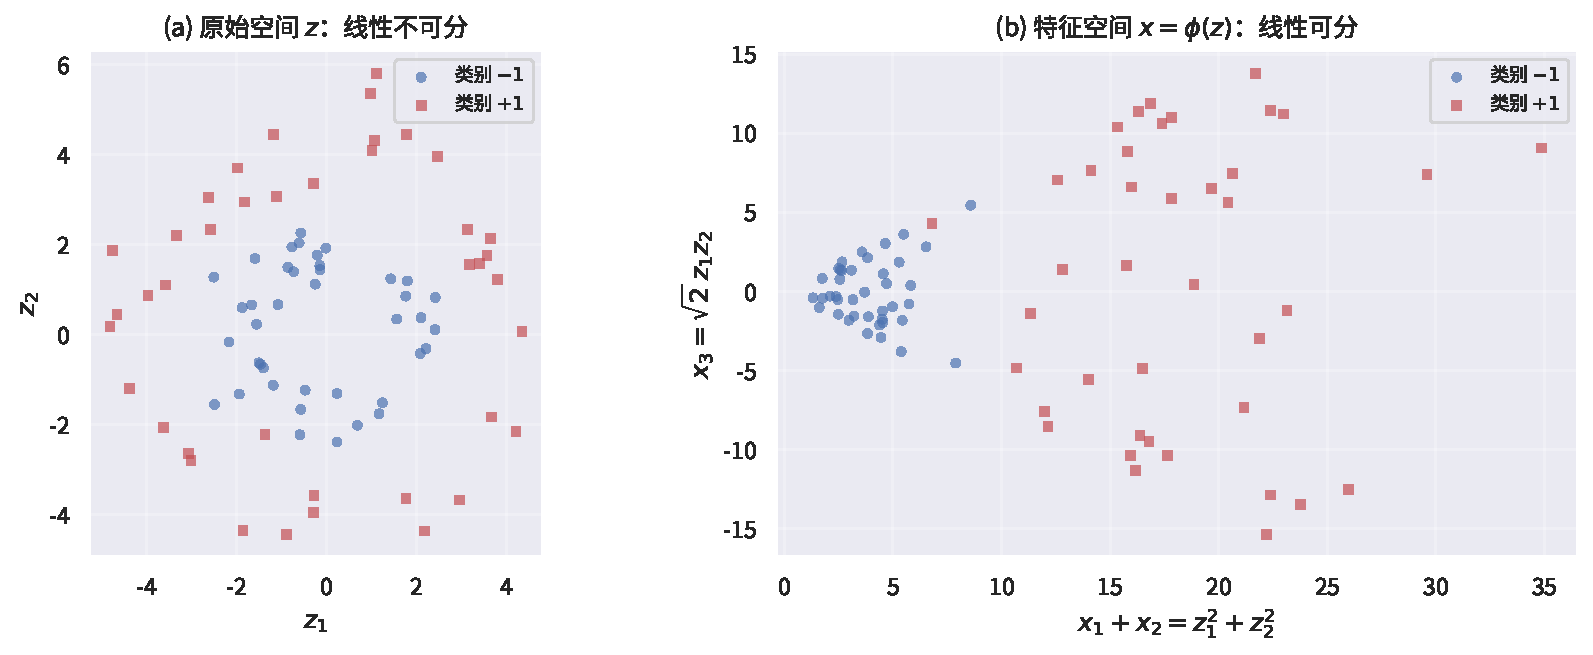
\includegraphics[width=\linewidth]{figures/ch7_kernel.pdf}
  \caption{核方法的几何本质：同一份环形数据（按半径分两类），在原始潜空间 $z$（左）里任何直线都分不开；经二次特征映射 $\phi(z)=(z_1^2, z_2^2, \sqrt{2}z_1z_2)$ 升到特征空间（右）后，一个线性函数即可分开。\textbf{对 $x$ 线性 $=$ 对 $z$ 非线性}——线性回归的预测由此成为潜空间中的天然非线性方法。}
  \label{fig:ch7-kernel}
\end{figure}

\subsection[从核回归到深度网络：Fourier 特征的 ridgeless 回归与 NTK]{从核回归到深度网络：ridgeless 回归、Fourier 特征与神经正切核}\label{sec:ntk}

本章最后做一件「收拢全书」的事：把「线性回归 $\to$ 核回归」这条路一直走到\textbf{深度神经网络}的门口。沿途有两座桥：第一座是\textbf{随机 Fourier 特征}（旧桥，2007），第二座是\textbf{神经正切核}（NTK，新桥，2018）\cite{jacot2018}。

\subsubsection*{桥一：两层网络 = 随机特征上的线性回归}

考虑最简单的两层网络
\begin{equation}\label{eq:two-layer}
  f(\bm{z}; \bm{a}) = \frac{1}{\sqrt{D}} \sum_{j=1}^{D} a_j\, \sigma\big( \bm{\omega}_j^\top \bm{z} + b_j \big),
\end{equation}
其中 $\sigma$ 是激活函数（ReLU、tanh 等），第一层参数 $(\bm{\omega}_j, b_j)$ 从某分布\textbf{随机采样后冻结}，只训练第二层 $\bm{a} \in \R^D$。注意两件事：

\begin{enumerate}[label=(\arabic*)]
  \item 定义 $\phi(\bm{z}) = \tfrac{1}{\sqrt{D}}\big(\sigma(\bm{\omega}_1^\top\bm{z}+b_1), \dots, \sigma(\bm{\omega}_D^\top\bm{z}+b_D)\big)^\top$，则 $f(\bm{z};\bm{a}) = \phi(\bm{z})^\top\bm{a}$——\textbf{它就是关于 $\bm{a}$ 的线性回归}，本章全部机器（正规方程、GD 精确解、push-through、核化判据）原封不动适用。
  \item 若 $\bm{a}$ 的初值取零且用梯度下降训练，第 \ref{sec:implicit} 章的隐式正则化分析说：它收敛到\textbf{最小范数}插值解——在 $\bm{a}$ 的 Euclidean 范数意义下。这就是\textbf{ridgeless 回归}（$\lambda \to 0^+$ 的 ridge，见练习 \ref{ex:ridge-dual}）：\textit{没有任何显式惩罚，插值解中范数最小的那个被 GD 自动选中}。
\end{enumerate}

由 \eqref{eq:kernel-interp}，其预测的核形式不变，只是核函数换成了\textbf{随机特征核}
\begin{equation}\label{eq:rf-kernel}
  k_{\mathrm{RF}}(\bm{z}, \bm{z}') = \frac{1}{D}\sum_{j=1}^D \sigma(\bm{\omega}_j^\top\bm{z}+b_j)\,\sigma(\bm{\omega}_j^\top\bm{z}'+b_j)
  \ \xrightarrow{D \to \infty}\ \E_{\bm{\omega}, b}\big[ \sigma(\bm{\omega}^\top\bm{z} + b)\,\sigma(\bm{\omega}^\top\bm{z}' + b) \big],
\end{equation}
这正是 Rahimi \& Recht 随机 Fourier 特征的理论核心（对移位不变核，取 $\sigma = \cos$ 与特定采样分布，\eqref{eq:rf-kernel} 精确重现高斯核）\cite{rahimi2007}。\textbf{一句话：冻结第一层、训练第二层、零初始化、梯度下降 $=$ Fourier 特征空间里的 ridgeless 回归。}

\subsubsection*{桥二：NTK——全部参数都训练时，函数空间仍是线性的}

桥一留了一个「不自然」的假设：第一层被冻结。如果\textbf{所有参数} $\bm{\theta} = (\bm{a}, \{ \bm{\omega}_j, b_j \})$ 都参与训练呢？参数空间的损失
\[
  L(\bm{\theta}) = \frac{1}{2}\sum_{i=1}^n \big( f(\bm{z}_i; \bm{\theta}) - y_i \big)^2
\]
关于 $\bm{\theta}$ 一般\textbf{非凸}——这正是深度学习「神秘」的出处。Jacot、Gabriel 与 Hongler 的关键观察是：别盯参数空间，盯\textbf{函数空间}。对训练集上的残差向量 $\bm{r}_t = \big( f(\bm{z}_i; \bm{\theta}_t) - y_i \big)_i$，链式法则给出
\begin{equation}\label{eq:ntk-flow}
  \frac{d\, f(\bm{z}; \bm{\theta}_t)}{dt}
  = \nabla_{\bm{\theta}} f(\bm{z}; \bm{\theta}_t)^\top \frac{d\bm{\theta}_t}{dt}
  = -\sum_{i=1}^n \underbrace{\big\langle \nabla_{\bm{\theta}} f(\bm{z}; \bm{\theta}_t),\ \nabla_{\bm{\theta}} f(\bm{z}_i; \bm{\theta}_t) \big\rangle}_{\Theta_t(\bm{z}, \bm{z}_i)} \, r_{t,i} ,
\end{equation}
其中
\begin{equation}\label{eq:ntk-def}
  \Theta_t(\bm{z}, \bm{z}') := \big\langle \nabla_{\bm{\theta}} f(\bm{z}; \bm{\theta}_t),\ \nabla_{\bm{\theta}} f(\bm{z}'; \bm{\theta}_t) \big\rangle
\end{equation}
称为\textbf{神经正切核}（Neural Tangent Kernel）。\eqref{eq:ntk-flow} 的形状你一定认得：它就是\textbf{函数空间里的核梯度下降}——与第 \ref{sec:gd} 章的 $\widehat{\bbeta}_{t+1} = \widehat{\bbeta}_t - \eta\,\X^\top(\X\widehat{\bbeta}_t - \y)$ 同构，只是「设计矩阵的内积」被换成了「参数梯度的内积」。

NTK 的惊人之处在于其\textbf{宽网络极限}：以 $\tfrac{1}{\sqrt{D}}$ 缩放（\eqref{eq:two-layer} 已如此），当宽度 $D \to \infty$ 时：

\begin{enumerate}[label=(\arabic*)]
  \item 初始化时 $\Theta_0$ 依大数定律收敛到一个\textbf{确定性核} $\Theta$（对两层网络可显式算出，见练习 \ref{ex:ntk}）；
  \item 训练\textbf{全程}中 $\Theta_t$ 保持不动（$\Theta_t \to \Theta$，不随 $\bm{\theta}_t$ 漂移）——参数走了很远，核纹丝不动；
  \item 于是 \eqref{eq:ntk-flow} 成为\textbf{线性}常微分方程 $\frac{df_t(\bm{z})}{dt} = -\sum_i \Theta(\bm{z},\bm{z}_i)\, r_{t,i}$，其解以 $\Theta$ 的特征方向指数收敛，极限为
  \begin{equation}\label{eq:ntk-ridgeless}
    f_\infty(\tilde{\bm{z}}) = \bm{\Theta}(\tilde{\bm{z}})^\top \bm{\Theta}^{-1} \y,
  \end{equation}
  其中 $\bm{\Theta} = \big(\Theta(\bm{z}_i,\bm{z}_j)\big)_{ij}$ 是 NTK 在训练点上的 Gram 矩阵，$\bm{\Theta}(\tilde{\bm{z}})$ 是新样本的核向量。
\end{enumerate}

\eqref{eq:ntk-ridgeless} 与本章的 \eqref{eq:kernel-interp} \textbf{逐符号同构}：无穷宽、全参数训练的两层（乃至任意深度\cite{lee2019}）神经网络，在梯度下降下的函数空间极限，就是\textbf{以 NTK 为核的 ridgeless 核回归}。参数空间的非凸性是一个「坐标系的幻象」——换到函数空间，深度网络训练就是第 5 章的最小范数插值故事。

\begin{keybox}[从一条直线到深度网络的桥]
\[
\begin{gathered}
\text{线性回归 } \xrightarrow{\ \phi\ } \text{ 核回归 } \xrightarrow[\text{显式化}]{\ \text{随机 Fourier 特征}\ } \text{ 有限维 ridgeless 回归} \\
\xrightarrow[\text{全参数训练、宽极限}]{\ \mathrm{NTK}\ } \text{ 深度网络的函数空间极限}
\end{gathered}
\]
四个箭头分别由本章第 \ref{sec:kernel-overdet} 节（push-through）、\eqref{eq:rf-kernel}（大数定律）、第 \ref{sec:implicit} 章（隐式正则化）与 \eqref{eq:ntk-ridgeless}（NTK 不动性）支撑。\textbf{线性回归不是深度学习的特例；深度学习的宽极限是线性回归的核化}——这就是为什么两百年前的这条直线，仍然是理解今天一切模型的最诚实的起点。
\end{keybox}

两点务实的注记。其一，NTK 描述的是「lazy training」\textit{懒惰训练} regime：参数初始化尺度大、训练位移小，网络「懒得」改变内部特征——真实深度学习中特征学习（feature learning）发生时 NTK 失效，此时理论仍在建设中（Jacot 本人区分 lazy regime 与 feature-learning regime 的后续工作即为此）。其二，ridgeless 插值\textbf{非但不坏、还可能更好}：Belkin 等人的 double descent 观察表明，现代过参数模型的测试误差在插值阈值之后继续下降\cite{belkin2019}——第 \ref{sec:minnorm} 章的最小范数解正是这一现象最干净的线性化身，Jingfeng Wu 等人的工作进一步证明最优提前停止的 GD 在统计意义下支配最优 ridge（见前言与文献）\cite{wu2025}。把这两条注记与 \eqref{eq:ntk-ridgeless} 放在一起，你就拿到了「为什么过参数化网络能泛化」这个问题的、目前最诚实的线性回答。

\begin{figure}[htbp]
  \centering
  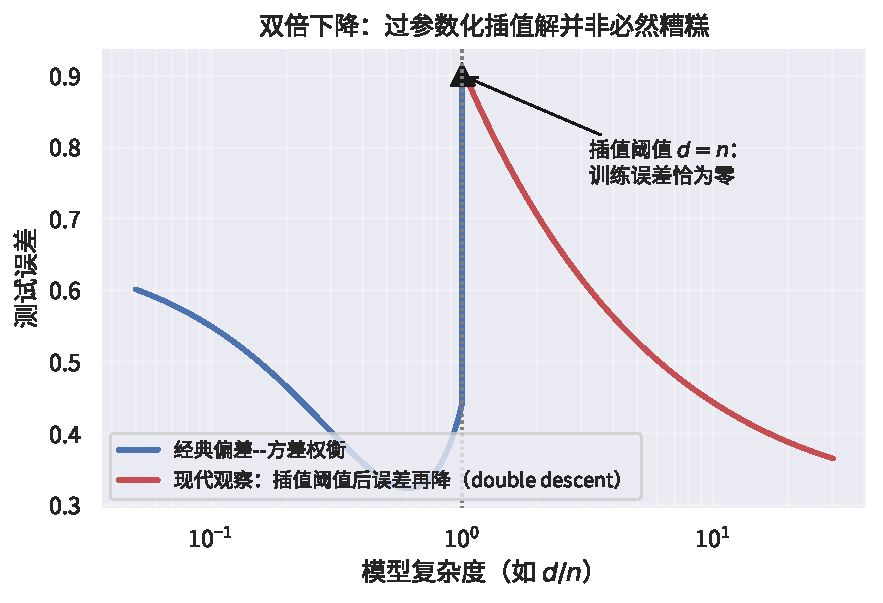
\includegraphics[width=0.72\linewidth]{figures/ch7_doubledescent.pdf}
  \caption{双倍下降（示意图；Belkin et al., 2019\cite{belkin2019}）：经典教科书说测试误差在 $d \approx n$ 处最优（蓝，U 型），现代观察发现误差在插值阈值 $d=n$ 处尖峰后\textbf{继续下降}（红）——插值本身不是罪，关键是插值解中隐式正则化选了哪一个。ridgeless 回归与提前停止的 GD 给出了这一选择的线性刻画。}
  \label{fig:ch7-doubledescent}
\end{figure}

\begin{exercise}\label{ex:ntk}
对 \eqref{eq:two-layer} 的两层网络（$\sigma$ 光滑），设 $(\bm{\omega}_j, b_j) \sim \mathcal{N}(\zero, \bm{I})$ i.i.d.，$\bm{a}$ 初值独立采样且 $\E[a_j^2] = 1$。验证：宽度 $D \to \infty$ 时，初始化处的 NTK \eqref{eq:ntk-def} 逐点收敛到
\[
  \Theta(\bm{z},\bm{z}') = \E\big[ \sigma(\bm{\omega}^\top\bm{z}+b)\,\sigma(\bm{\omega}^\top\bm{z}'+b) \big] \;+\; \bm{z}^\top\bm{z}'\, \E\big[ \sigma'(\bm{\omega}^\top\bm{z}+b)\,\sigma'(\bm{\omega}^\top\bm{z}'+b) \big],
\]
并指出两项分别来自「最后一层参数」与「第一层参数」的梯度；再说明第二项（随机特征核 \eqref{eq:rf-kernel} 中没有的那一项）为何使 NTK 严格强于随机特征核。对 $\sigma = \mathrm{ReLU}$，利用正态分布的半空间矩公式把两个期望写成 $\bm{z}$、$\bm{z}'$ 角度的显式函数。
\end{exercise}

\subsection{本章结论}\label{sec:kernel-conclusion}

\begin{keybox}[要点]
\begin{itemize}
  \item 设 $\x_i = \phi(\bm{z}_i)$，记 $\bm{K}_{ij} = k(\bm{z}_i,\bm{z}_j)$、$\bm{k}(\tilde{\bm{z}})_i = k(\tilde{\bm{z}}, \bm{z}_i)$，则
  \[
    d > n:\ \tilde{\x}^\top \widehat{\bbeta}' = \bm{k}(\tilde{\bm{z}})^\top \bm{K}^{-1} \y
    \ \xrightarrow{\ \lambda\ }\ 
    n \gg d:\ \tilde{\x}^\top \bhat^{\mathrm{ridge}} = \bm{k}(\tilde{\bm{z}})^\top (\bm{K} + \lambda \bm{I})^{-1} \y .
  \]
  线性回归的两个闭式解，都是\textbf{只用核函数组装的估计量}；
  \item 核化的关键两步：内积化（所有量写成 $\langle\phi,\phi\rangle$）与 push-through（$(\bm{\Phi}^\top\bm{\Phi} + \lambda\bm{I})^{-1}\bm{\Phi}^\top = \bm{\Phi}^\top(\bm{K} + \lambda\bm{I})^{-1}$）——后者把特征空间的逆翻转为样本空间的逆；
  \item 预测 $\hat{f}(\tilde{\bm{z}}) = \sum_i \alpha_i k(\tilde{\bm{z}}, \bm{z}_i)$ 对潜变量 $\bm{z}$ 是\textbf{非线性}的，尽管它对 $\x = \phi(\bm{z})$ 是线性的——「线性回归的预测是非线性潜空间映射下的天然核方法」，至此证毕；
  \item $d = \infty$（高斯核）时核化从便利变为必需；随机特征则反向地把核近似回有限维线性代数，连通过参数化网络。
\end{itemize}
\end{keybox}

\begin{exercise}\label{ex:kernel-dual}
用 \eqref{eq:push-through} 证明核岭回归的原始形式与对偶形式给出\textbf{完全相同}的预测函数，并解释为何 $\lambda > 0$ 时无需任何秩假设。
\end{exercise}

\begin{exercise}\label{ex:kernel-interp}
验证高斯核矩阵 $\bm{K}$（样本互异时）正定可逆，从而 \eqref{eq:kernel-interp} 有定义；进一步验证 \eqref{eq:kernel-expansion} 中的 $\bm{\alpha}$ 满足 $\bm{K}\bm{\alpha} = \y$（核插值方程），并把它与第 \ref{sec:gd-underdet} 章的插值验证 \eqref{eq:interp} 对应起来。
\end{exercise}
